\section*{}

	\begin{frame}
		\frametitle{Conclusion}
		
		\begin{center}
		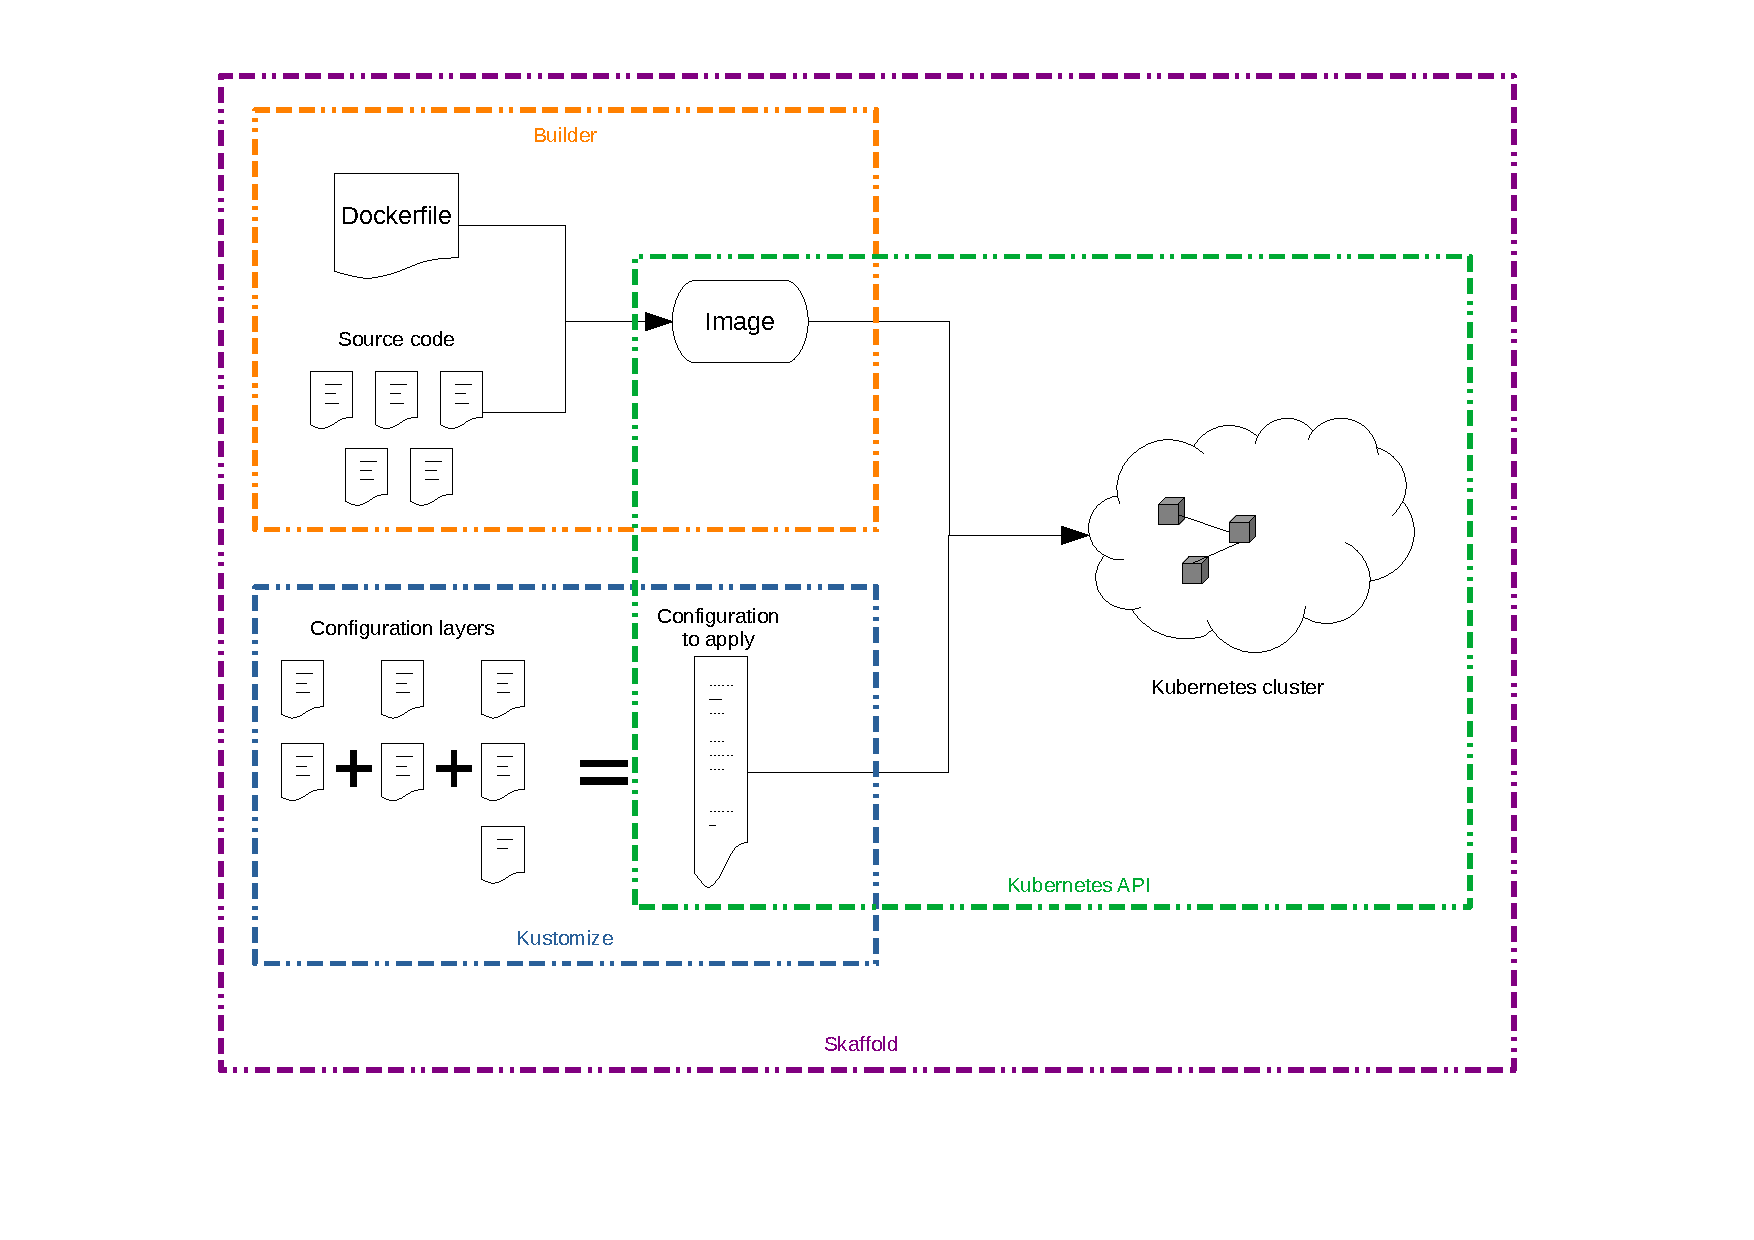
\includegraphics[height=6.8cm]{../../../resources/color/skaffoldKustomizeArchitecture.pdf}
		\end{center}
		
	\end{frame}
	
\subsection{Going further}
	\begin{frame}
		\frametitle{Going further?}
		
		With these tools it is possible:
		\begin{itemize}
			\item[$\bullet$] to use an other image builder than docker
			\item[$\bullet$] to have stacks with multiple images
			\item[$\bullet$] to use alk kind of kubernetes cluster instead of minikube
			\item[$\bullet$] to debug inside deployed containers
		\end{itemize}
	\end{frame}
	
	\begin{frame}
		\frametitle{A little more complex example}
		
		In \href{https://github.com/Tinkou/kubercoins}{this github repository}, you can found an example consisting of a complete stack.
		
		\bigskip
		
		This is an educational project based on \href{https://github.com/jpetazzo/dockercoins}{the work of jpetazzo}.
		
		\medskip
		
		This application stack is composed of 3 micro services, a redis database and a web UI. It generate and hash some random bit before counting the amount of bit groups hashed. The web UI display the average value.
		
	\end{frame}
	
	\begin{frame}
		\frametitle{A little more complex example}
		
		This project is useful to demonstrate the usage of several languages and to manipulate kubernetes configuration.
		
		\medskip
		
		Finally, in the branch \textit{exercise}, there is the base configuration and it is possible to use it to try to create kustomize and skaffold configurations.
	\end{frame}